\documentclass[
twocolumn,
% hf,
]{ceurart}

\sloppy

\usepackage{listings}
\usepackage{todonotes}
\usepackage{placeins}
\lstset{breaklines=true}
\usepackage{flushend}

\usepackage[absolute,overlay]{textpos}

\begin{document}

\copyrightyear{2024}
\copyrightclause{2024 Copyright for this paper by its authors. Use permitted under Creative Commons License Attribution 4.0 International (CC BY 4.0).}

\conference{CLiC-it 2024: Tenth Italian Conference on Computational Linguistics, Dec 04 — 06, 2024, Pisa, Italy}

\title{You write like a GPT}

\author[1]{Andrea Esuli}[%
orcid=0000-0002-5725-4322,
email=andrea.esuli@isti.cnr.it,
]
\author[1]{Fabrizio Falchi}[%
orcid=0000-0001-6258-5313,
email=fabrizio.falchi@isti.cnr.it,
]
\author[1,2]{Marco Malvaldi}[%
%orcid=0000-0000-0000-0000,
%email=@,
]
\author[1]{Giovanni Puccetti}[%
orcid=0000-0003-1866-5951,
email=giovanni.puccetti@isti.cnr.it,
]

\fnmark[1]

\address[1]{Istituto di Scienza e Tecnologie dell'Informazione ``A. Faedo''- Consiglio Nazionale delle Ricerche}
\address[2]{Professional writer}

\fntext[1]{All the authors contributed equally.}

%%%%%%%%%%%%%%%%%%%%%%%%%%%%%%%%%%%%%%%%%%%%

\begin{abstract}
We investigate how Raymond Queneau's \textit{Exercises in Style} are evaluated by automatic methods for detection of artificially-generated text.
We work with the Queneau's original French version, and the Italian translation by Umberto Eco.

We start by comparing how various methods for the detection of automatically generated text, also using different large language models, evaluate the different styles in the opera.
We then link this automatic evaluation to distinct characteristic related to content and structure of the various styles.

This work is an initial attempt at exploring how methods for the detection of artificially-generated text can find application as tools to evaluate the qualities and characteristics of human writing, to support better writing in terms of originality, informativeness, clarity.
\end{abstract}

%%%%%%%%%%%%%%%%%%%%%%%%%%%%%%%%%%%%%%%%%%%%

\begin{keywords}
GPT \sep
style \sep
generated text \sep
human writing
\end{keywords}

%%%%%%%%%%%%%%%%%%%%%%%%%%%%%%%%%%%%%%%%%%%%

\maketitle

%%%%%%%%%%%%%%%%%%%%%%%%%%%%%%%%%%%%%%%%%%%%

\section{Introduction}

The extraordinary writing ability of the latest chatbots and virtual assistants based on Large Language Models (LLMs) poses a significant question for anyone who attempts to write today —- be they a scientist, a writer, or a lover: is it worth the effort to engage in the act of writing?

For those not hindered by excessive laziness and who, with courage, still tackle writing with determination and passion, this question implies a more specific one: am I writing a text that an artificial intelligence could not have produced?

We believe that the answer to this question may, in the future, come from the LLMs themselves given that they are designed to assess the probability of the occurrence of the next word in a text. 
We envision a future where LLMs, although widely used to produce essentially obvious texts, will assist those who still engage in writing to create texts worth reading, if only because the artificial intelligence, having read and statistically evaluated almost everything ever written, considers them non-obvious and distinct from what it would have produced itself.

The ability of LLMs to evaluate the probability of the next word in a text stems from the extensive corpus of writing they are trained on. 
Consequently, their evaluation of a piece of writing is ultimately based on an indirect comparison between the given text and the entire body of literature they have been exposed to. 
Using LLMs to assess how much a text differs from the production capabilities of LLMs inherently implies an evaluation of the novelty it represents compared to known literature.

Starting to move in this direction, this article explores whether an LLM can be used to help humans answer this question. 
In this first attempt we do this not based on the content intended for communication but on the style. 
We have conducted a preliminary study on the possibility of using LLMs to evaluate how and to what extent a certain writing style and/or a specific text differs from what a machine can achieve.

We took as a reference Raymond Queneau's ``Exercises in Style'' \cite{queneau1947exercises}, which draws from Erasmus of Rotterdam's ``De Utraque Verborum ac Rerum Copia'' \cite{erasmus1512} a bestseller widely used for teaching how to rewrite pre-existing texts and how to incorporate them into a new composition. 
In Queneau's work, the same simple story is revisited each time in a different literary style. 
We asked ourselves and conducted experiments on how much the texts in various styles used by Queneau differ from the writing abilities of LLMs, which have acquired their skills by learning statistical relationships from vast amounts of text.

Calvino had already attempted to answer this question: ``What would be the style of a literary automaton?''
He replied, ``The test for a poetic-electronic machine will be the production of traditional works, of poems with closed metric forms, of novels with all the rules''. 
We believe it has indeed happened this way, as today's chatbots and virtual assistants are built from a language model.

In this work, we provide initial evidence that language models  recognize those texts that are more traditional, particularly used in spoken language or by classical characters as more probable while they deem more unlikely experimental and innovative texts. However, we find evidence that even for powerful LLMs it remains difficult to cut a clear line between experimental texts and those that instead incur the risk of becoming unreadable. 

%%%%%%%%%%%%%%%%%%%%%%%%%%%%%%%%%%%%%%%%%%%%

\section{Related Work}

The evaluation of text readability may dated back at least to the work of Flesch in 1948 \cite{flesch1948new}. Flesch's method was based on simple surface properties of text (i.e., words per sentence and syllables per word).
Since then a steady evolution of methods involved more complex NLP and ML as new tools were developed (see the surveys \cite{collins2014computational, vajjala2021trends}).

An example of the use of LLMs on this topic is the work \citet{Miaschi20}, which investigated the correlation between a readability score measured by an automatic readability tool (READ-IT \cite{DellOrletta11}) and the perplexity measured by an LLM, yet they found no significant correlation between the two dimensions.

\citet{hayati2021does} compared human and BERT-based relevance scoring of words in a sentence to determine its style, polite or offensive, as well as the expression of sentiment and emotions.
They found a loose correlation in the way words are identified as relevant by humans and BERT, with BERT giving more relevance to context word (e.g. ``baseball'' for the emotion of joy), while human are more focused on words perceived as ``typical'' of the style. (e.g., ``smile'' for joy).

The style transfer process is the task of rewriting a passage of text changing the set of lexical choices and syntactic structures, yet not substantially changing the actual content of the text.
\citet{krishna-etal-2020-reformulating} surveys the style transfer literature and proposed a style transfer method trained on reconstructing a style-specific text (inverse paraphrase) on pseudo-parallel data generated using a diverse paraphrase model.

\citet{qi-etal-2021-mind} proved that a change of the writing style, made using a trained model, can be an effective means of attack to BERT-based classifiers, e.g., letting an offensive text be classified as non-offensive just by rewriting it using a Bible-like style.
Similarly \citet{krishna23} have shown that automatic paraphrasing can be extremely effective at breaking the ability of detection method to recognize artificially generated text.

%%%%%%%%%%%%%%%%%%%%%%%%%%%%%%%%%%%%%%%%%%%%

\section{Writing with style}
\label{sec:queneau}

\begin{figure}[t]
    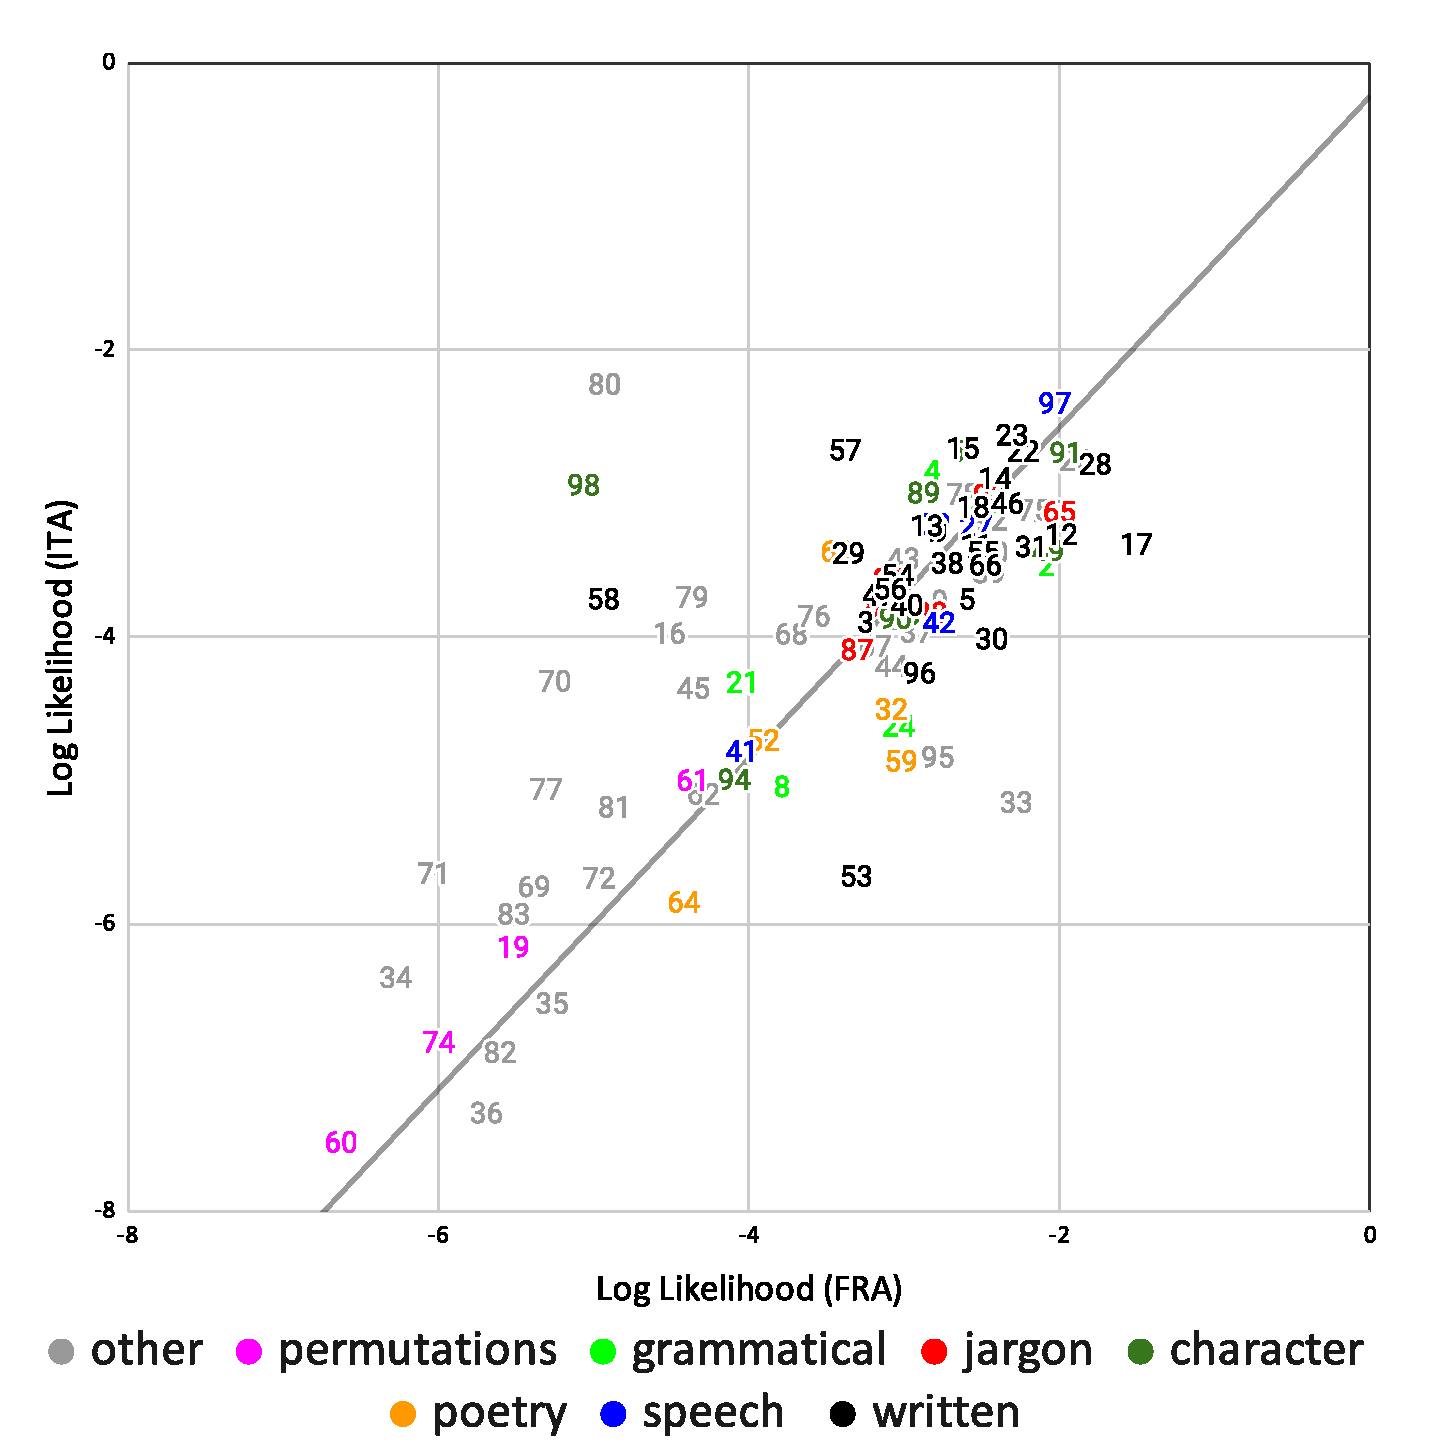
\includegraphics[trim=0.5cm 0cm 0.5cm 0.5cm, clip, width=\columnwidth]{LL-trend.pdf}
    \centering
    \caption{Log Likelihood for both the Italian and French versions of ``Exercises in Style''. The numbers provided correspond to the IDs in Table \ref{tab:megatable}. The colors indicate the exercise group. The line show the correlation ($R^2=0.805$).}
    \label{fig:ll_corr_ita_fra}
\end{figure}

\begin{table*}[!ht]
    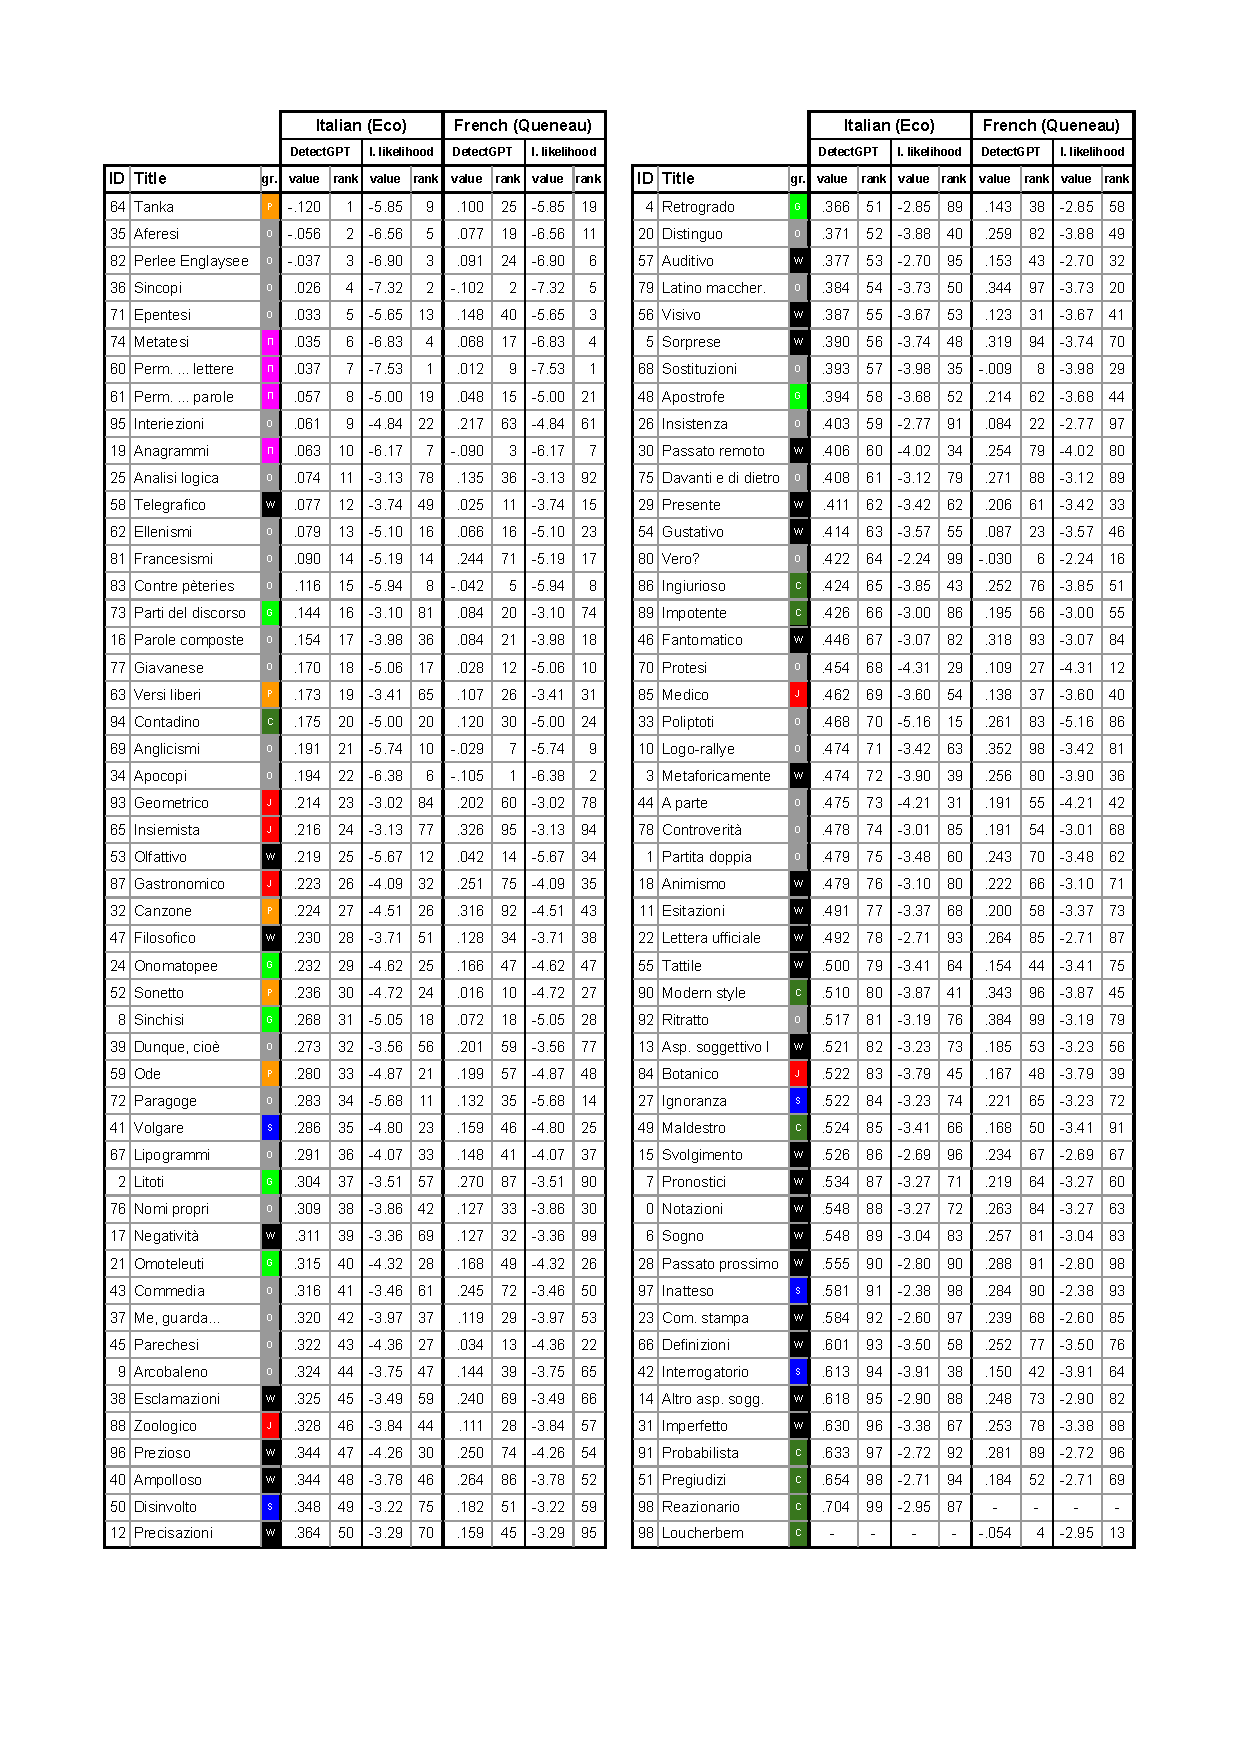
\includegraphics[width=\textwidth]
    {Table.pdf}
    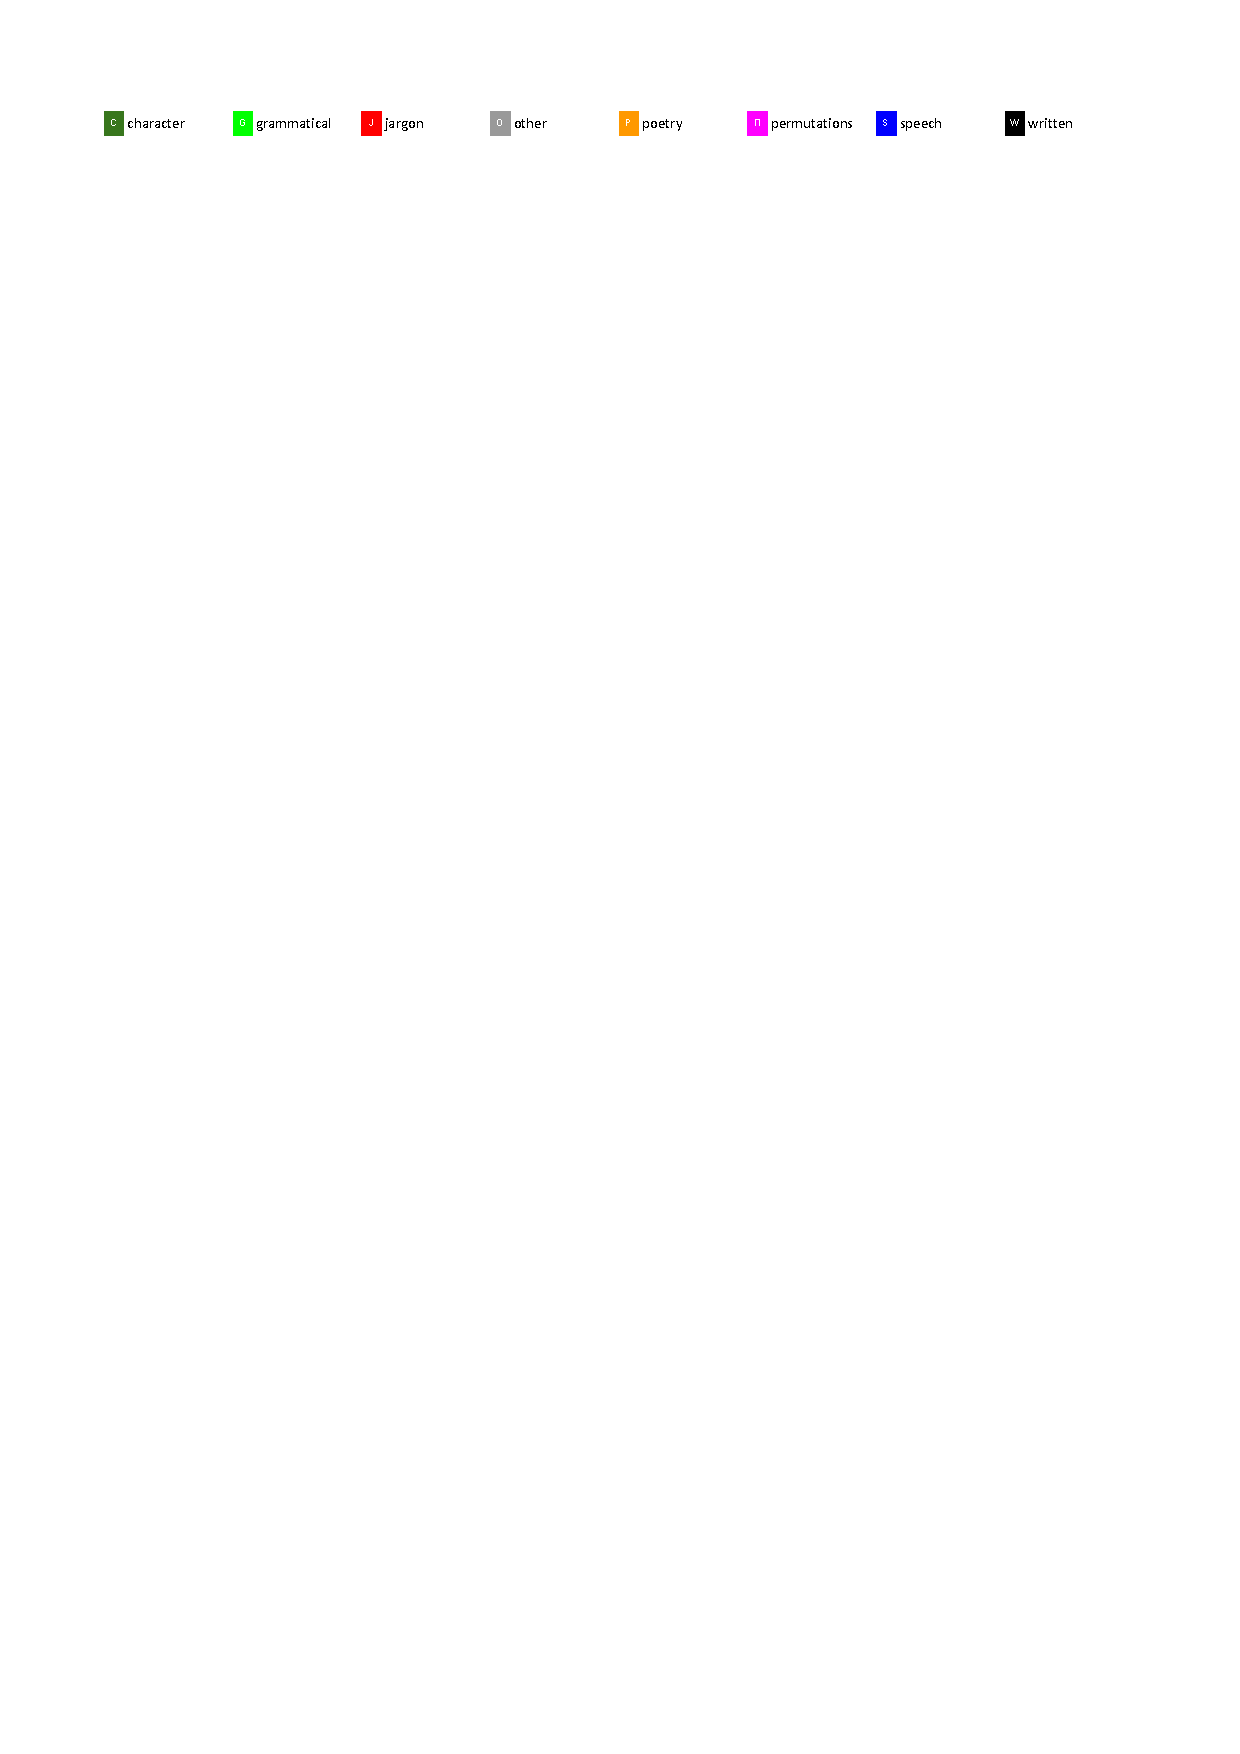
\includegraphics[width=\textwidth]
    {legend.pdf}
    \centering
    \caption{Scores and ranks of the various styles with respect to various detection methods.
    Styles are ranked by the DetectGPT score on Italian. Groups are indicated by their initials (\( \Pi \) is used for \emph{permutations}) and are color-coded consistently with the previous figures.}
    \label{tab:megatable}
\end{table*}

Queneau's original work in French of 1947 \cite{queneau1947exercises} tackles on telling the same short story using 99 different styles.
The first style, Notations, is a clear report of a sequence of events, each with details that together define the actual content of the story that is reported in all of the other 98 versions.
Each version has a defining title that denotes its style.
Styles can be grouped by similarity; Barbara Wright, who made the English translation in 1958  \cite{queneau1958exercises}, reports to have roughly identified seven groups\footnote{In the preface of the book where the groups are listed, Wright did not report a complete assignment of all styles to these groups, only hinting a few cases for some of them.}:
\begin{itemize}
    \item different types of speech;
    \item different types of written prose, e.g.,  Official Letter, Philosophic;
    \item five poetry styles, e.g., Haiku, Ode;
    \item eight language-based character sketches, e.g., Reactionary, Biased, Abusive;
    \item grammatical and rhetorical forms, e.g., Litotes, Synchesis, Parts of speech;
    \item jargon, e.g., mathematical, botanical;
    \item and the very specific group of Permutations, by groups of letters or words.
\end{itemize}
Along time, new editions presented variations in the list of styles. 
For example, five styles in the original edition\footnote{R\'eactionnaire, Feminine, Hai-Kai, Permutations de 2 \'a 5 lettres, Permutations de 9 \'a 12 lettres.}, were replaced by other five in the edition of 1969\footnote{Ensembliste, D\'efinitionnel, Tanka, Translation, Lipogramme.}, the one we used in our experiments. 

Queneau's opera has been translated in more than 30 languages.
The Italian translation was made by Umberto Eco \cite{queneau1983esercizi}, in 1983.
Similar to other translations, the Italian translation reports almost all the original styles, but some are considered untranslatable and replaced with variants semantically similar to the original ones, or relevant for other reasons.
For example the style Homophonique was replaced by Eco with a style named Vero? (True?), because French has many homophones while Italian has not. 
The Vero? style links to the repeated use of intercalation and links to the Alors style of the French edition.
Eco also decided to not translate the Loucherbem style, based on the slang spoke by Parisian and Lyonnaise butchers, considering not interesting to link it to an Italian slang or dialect, whereas dialect-based styles already were included in the opera.
Eco replaced it with its own version of the R\'eactionnaire style from the first edition, which he liked more, as he detailed in the preface of his translation.

%%%%%%%%%%%%%%%%%%%%%%%%%%%%%%%%%%%%%%%%%%%%

\section{Style and detection, is there a relation?}

\begin{figure}[t]
    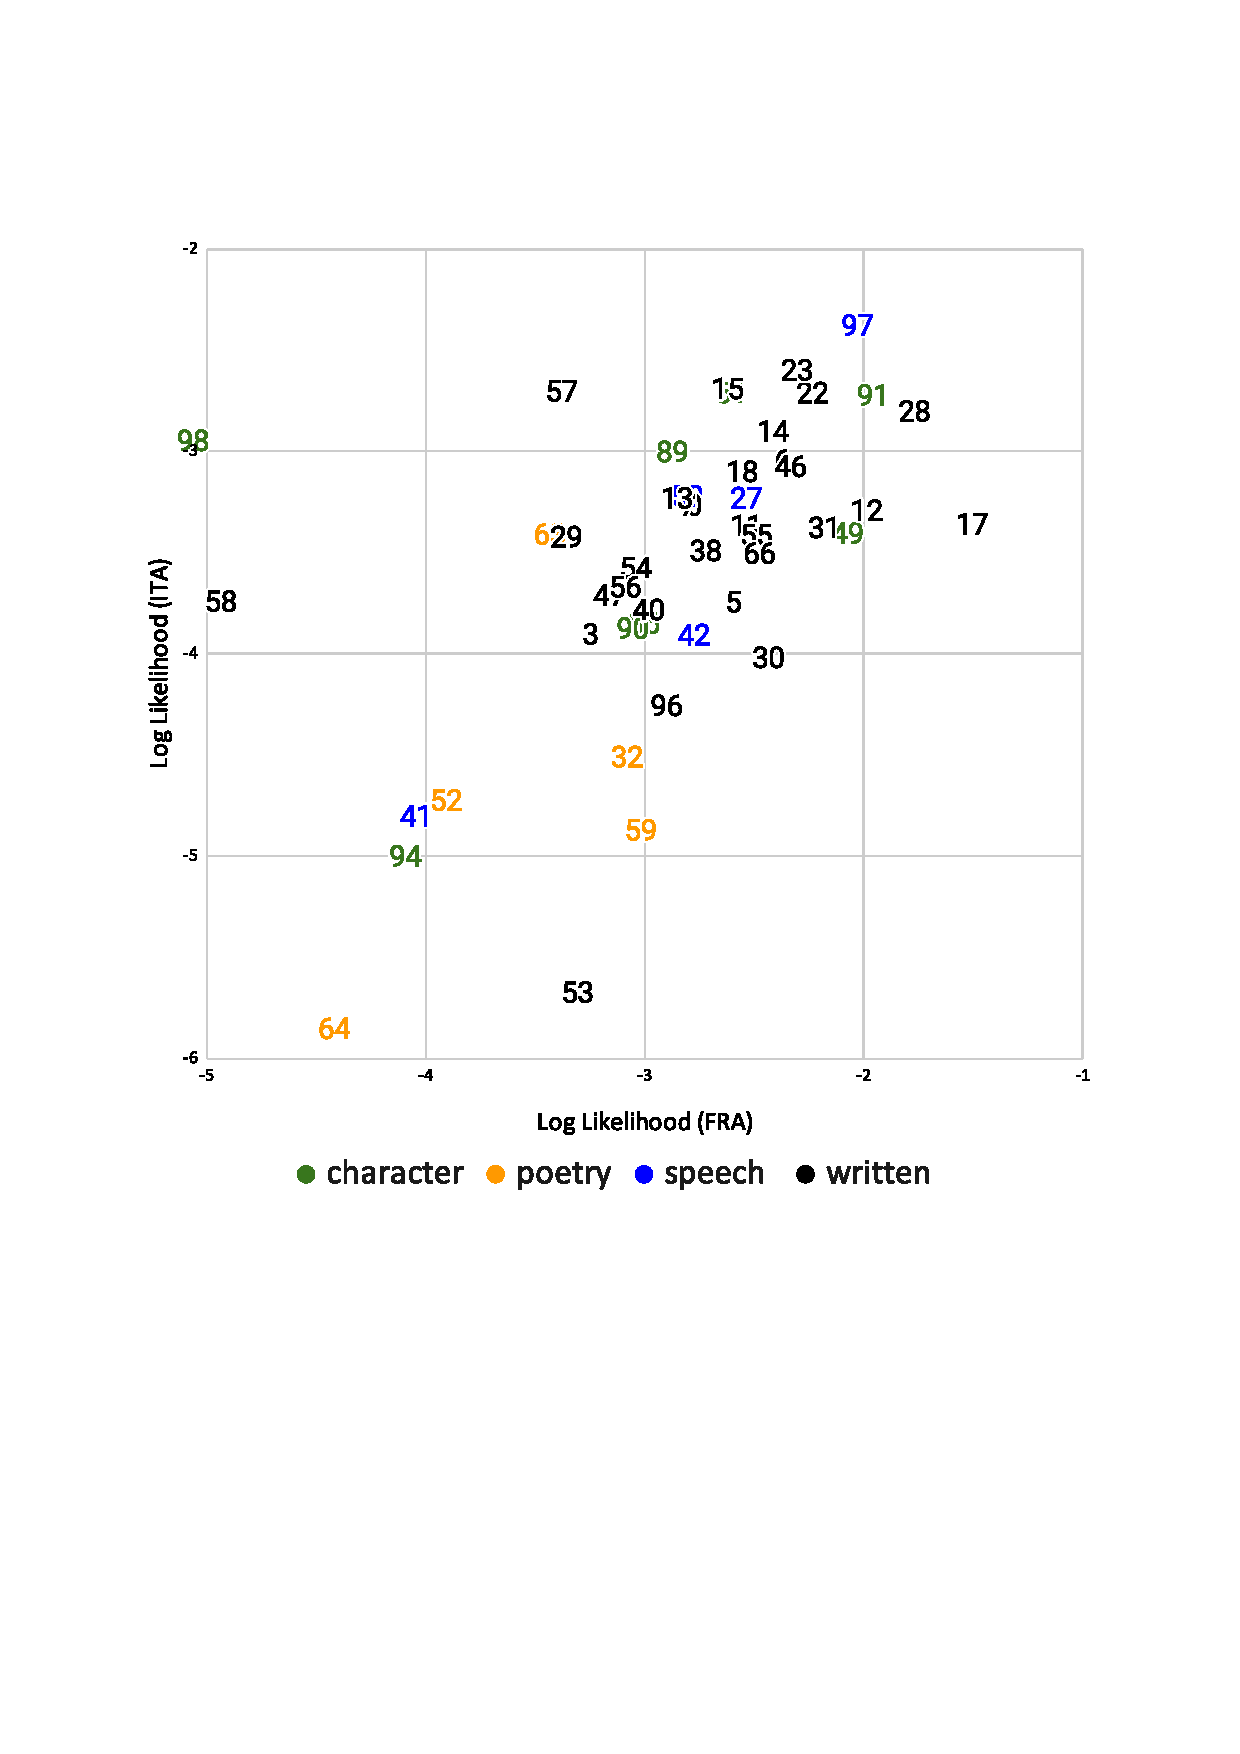
\includegraphics[trim=0.5cm 0cm 0.5cm 0.5cm, clip, width=\columnwidth]{LL-zoom.pdf}
    \centering
    \caption{Log Likelihood for the main groups, presented in a zoomed-in view.}
    \label{fig:ll_corr_ita_fra_zoom}
    
\end{figure}

\begin{figure}
    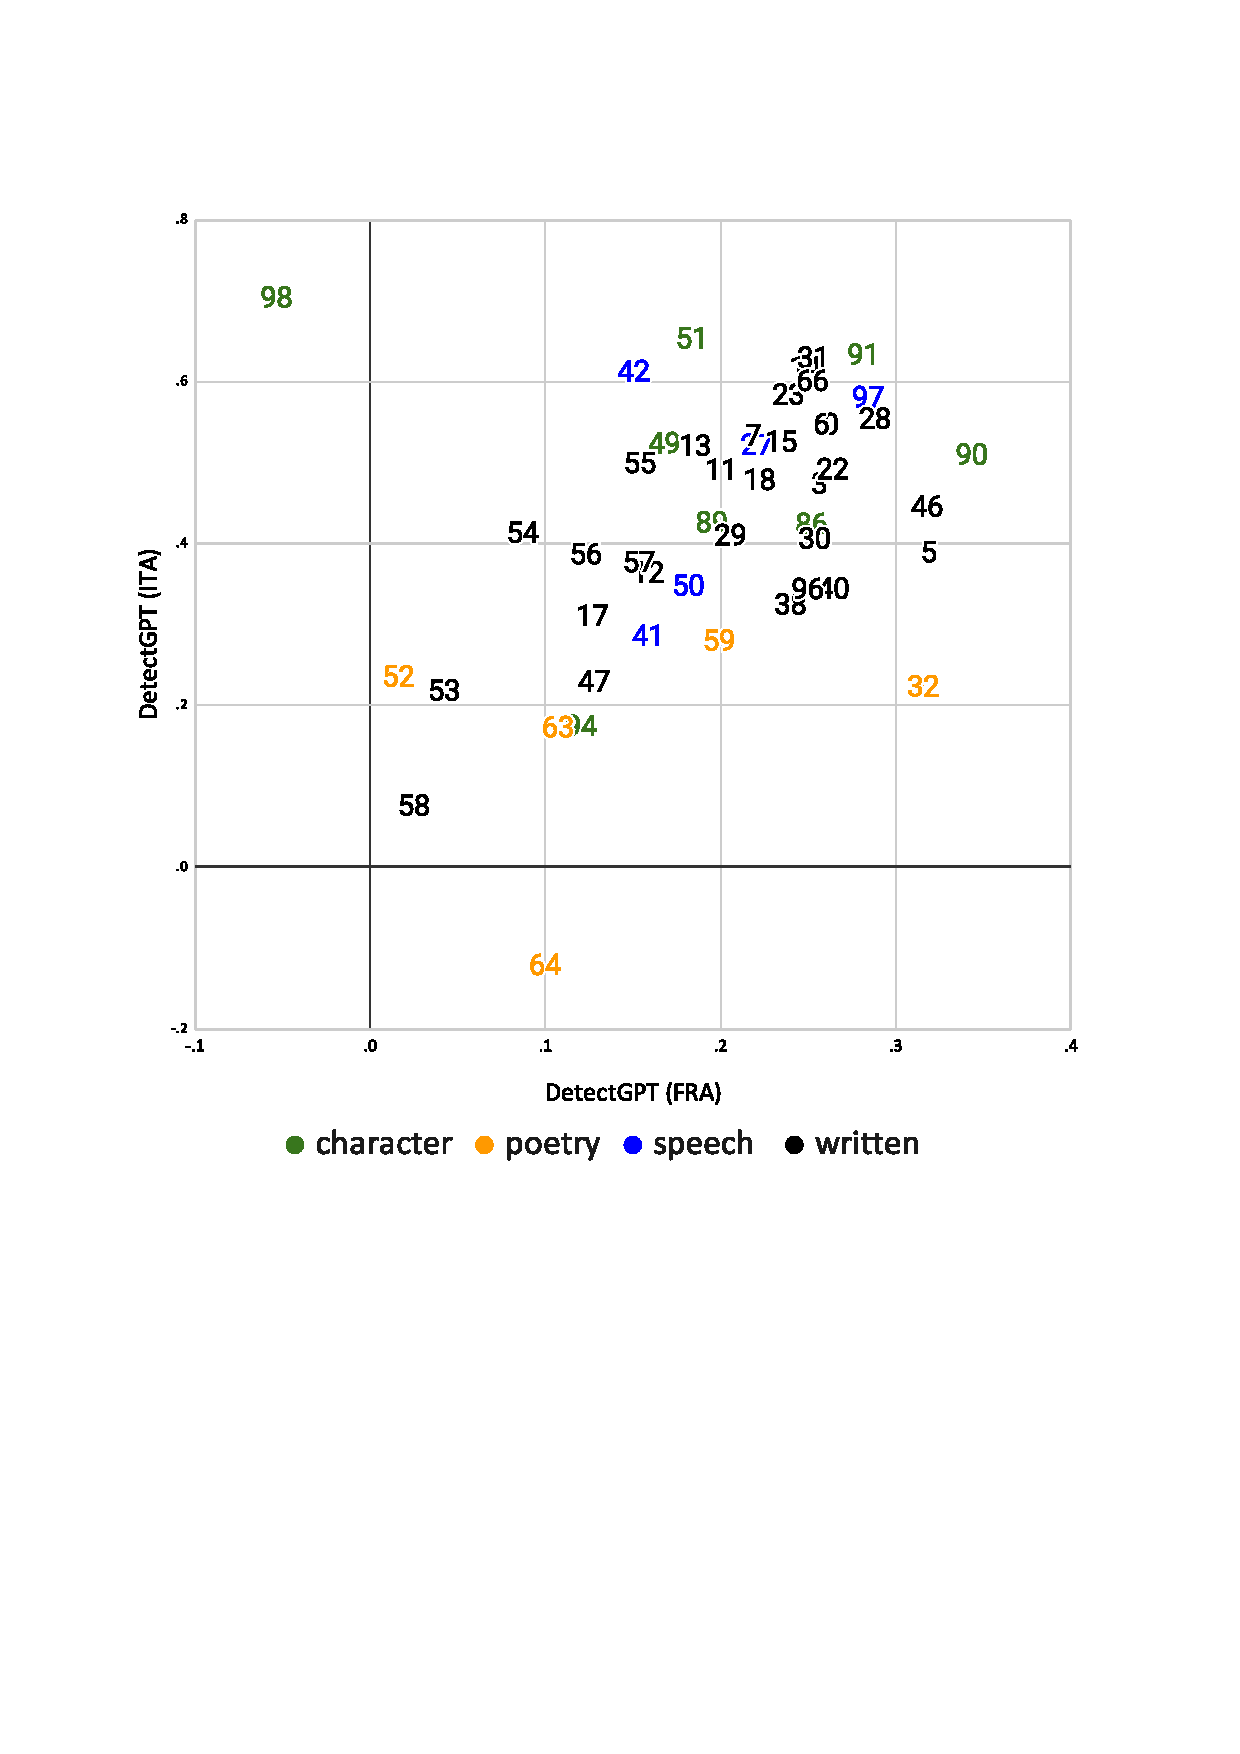
\includegraphics[trim=0.5cm 0cm 0.5cm 0.5cm, clip, width=\columnwidth]{DetectGPT-zoom.pdf}
    \centering
    \caption{DetectGPT scores for the main groups.}
    \label{fig:dgpt_corr_ita_fra_zoom}
\end{figure}


The Research Question (RQ) we wish to answer is the following:
\textbf{Can we use Machine Generated Text (MGT) detection methodologies to measure some qualities and characteristics of the style used in writing a piece of text?}

Our assumption supporting the relevance of this RQ is that LLMs, trained on trillions of tokens, naturally approximate an \emph{average writing style} that is necessarily ``average'' and thus not original or unique. 
On the other hand, original and surprising writing styles, which by definition will come in many very different forms, will be less frequent, and sparse across the long tail in the distribution of training data, and thus modeled as less likely according to the LLMs.

We use two metrics to measure the style of texts according to language models, \emph{Log Likelihood} (LL) and \emph{DetectGPT} \citep{mitchell_detectgpt_2023}, these metrics are used to detect text generated by a given language model since on average they will be higher for text that a language model has generated, when compared to text written by a human.

We focus on Eco's Italian and Queneau's original French versions of the style exercises. 
To measure the scores, we use LLMs tuned for these languages. 
For Italian we use Anita \cite{polignano2024advancednaturalbasedinteractionitalian} while for French Mistral \cite{jiang2023mistral}. 

As a first validation of our assumption, Figure \ref{fig:ll_corr_ita_fra} shows the correlation between the \emph{Log Likelihood} each writing style passage is assigned in Italian (y-axis) and in French (x-axis). The Figure shows significant correlation and zooming in on the higher \emph{Log Likelihood} texts, Figure \ref{fig:ll_corr_ita_fra_zoom}, we see that the correlation persists.

Similar results hold for \emph{DetectGPT}, Figure \ref{fig:dgpt_corr_ita_fra_zoom}, shows the correlation between this score for the Italian texts and for the French ones, and the correlation is close to the one for \emph{Log Likelihood} shown in Figure \ref{fig:ll_corr_ita_fra_zoom}.

Both Figures \ref{fig:ll_corr_ita_fra_zoom} and \ref{fig:dgpt_corr_ita_fra_zoom} show style number 98 as a kind of outlier.
This is a correct measurement as style 98 is actual two different styles between the two versions, Loucherbem in French, and Reazionario in Italian, as reported in Section \ref{sec:queneau}.

Both \emph{Log Likelihood} and \emph{DetectGPT} appear to behave consistently across languages and styles, supporting our hypothesis that some characteristics of the writing styles are captured by these scores. 

\subsection{Analysis of Detection Scores of Styles}

Table \ref{tab:megatable} shows the actual value of \emph{Log Likelihood} and \emph{DetectGPT} for each passage in both Italian and French as well as their ranking among all style exercises, ranked based on the \emph{DetectGPT} score in Italian.
We adopted Wright's grouping of styles, assigning each style to one of the seven groups listed in Section \ref{sec:queneau}, and also adding an ``other'' group for styles for which we could not find a clear positioning in Wright's groups (typically the styles based on almost obsessive repeated use of some kind of expression).
The (colored) \emph{gr.} column reports the style group that is assigned to each style exercise and we can observe that ranking the styles based on the \emph{DetectGPT} scores in Italian (as they are reported in the table) highlights a few prominent patterns which we now describe.

The \textbf{\emph{permutation}} class is present only in the lower ranks, and indeed the texts belonging to this group are hard to read and don't show any recognizable stylistic pattern, they are more akin to games that makes sense only within the context of Queneau's book.

The texts belonging to the \textbf{\emph{jargon}} are mostly in the lower end of the tail. 
The styles that are in higher ranks are likely to be present in higher quantity in LLMs training data justifying the ranking shift.

The \textbf{\emph{poetic}} class is the next one in average rank, just higher than the \emph{permutation} one, with the exception of the "Tanka" style, which is indeed a very short text, with almost no syntax connecting minimal sentences.

Interestingly, right above the \emph{poetic} group stands the \textbf{\emph{grammatical and rhetorical}} group; indeed rhetorical figures are a key component of poem writing. This group is evenly spread among the middle ranks, with the exception of ``Parti del discorso'' (Part of speech), which is in a lower position, and which also the one with more loose relation with \emph{grammatical and rhetorical} group.

The \textbf{\emph{writing}} group, contains a large number of styles and is spread across several ranks, however it is heavily skewed towards the higher ranks.

The \textbf{\emph{speech}} group is entirely in the higher ranks and as its spoken source suggests it has a strong character-rooted component.

Accordingly, the only group that ranks higher than \emph{speech} is \textbf{\emph{character}}\footnote{Character as in ``the character of a play''.} which, with only two exceptions, ``Ingiurioso'' (Offensive) and ``Impotente'' (Powerless), always ranks in the top quarter, takes all 3 top ranks and is the highest ranking one.
The last line of Table \ref{tab:megatable} reports the ranks and scores for the Loucherbem style, which exists only in the French version. The ranks are very low as this style uses almost made up words to replicate the phonetics of the jargon.

The \textbf{\emph{other}} group which contains all those styles which are harder to assign to a specific group is evenly spread across the lower ranks with few exceptions indicating that the texts that compose it are indeed quite varying and hard to group together.

An overall look at the ranking without considering the groups suggests a relation between the scores of detection methods and some characteristics of the styles.
Styles that make use of unusual, or just made up words, or do not use a correct syntax, get low detection scores. 
Styles that are based on a clean, modern prose, with a simple syntax, get high detection scores. 
The middle ranks show a smooth transition among the two extremes, in which the use of unusual terms or syntax is more frequent as the detection scores get lower.

%%%%%%%%%%%%%%%%%%%%%%%%%%%%%%%%%%%%%%%%%%%%

\section{Conclusions}

This work is a first exploration of the idea of designing tools that evaluate how and to what extent a writing style and/or a specific text differs from what a machine can achieve.
We tested for this task the use machine generated text detection tools, under the hypothesis of a correlation between their detection scores and our goal of discovering the many facets that build an original human written text.
We applied them to Queneau's exercises in style, in which the same story is written using a rich and varied set of writing styles.
We have found a consistent correlation between the scores assigned by detection methods, across detection methods and across languages.

The comparison of the styles with their detection scores indicates that lower scores from detection methods are correlated with the use of unusual terms or syntax, while higher scores are more related to styles that are based on a clean and more prose, with a smooth transition among this two extremes.
The ranks thus do not indicate a ``better'' or a more ``interesting'' style, yet they confirm Calvino's statement we reported in the introduction: content that is akin to a machine-generated one is the one that produce ``traditional'' content, following the main rules of writing.

Writers willing to depart from sounding ``ordinary'' could indeed use detection methods to estimate these aspects on their content, with the caveat that while a mid-level detection score may suggest some original traits in text, low scores may not indicate a more original or interesting text, but they may likely derive from an obscure or plainly unreadable text.

Given the positive results of this first investigation, future developments will be based on the use of texts specifically written for this activity. This will have the advantage of having full control over the contents and to have the guarantee that they have never been part of the LLMs training data.

\FloatBarrier

%%%%%%%%%%%%%%%%%%%%%%%%%%%%%%%%%%%%%%%%%%%%

\begin{acknowledgments}
This work was partially supported by PNRR - M4C2 - Investimento 1.3, Partenariato Esteso PE00000013 - "FAIR - Future Artificial Intelligence Research" - Spoke 1 "Human-centered AI", funded by European Union - NextGenerationEU.
\end{acknowledgments}

%%%%%%%%%%%%%%%%%%%%%%%%%%%%%%%%%%%%%%%%%%%%

\bibliography{biblio,custom}

%%%%%%%%%%%%%%%%%%%%%%%%%%%%%%%%%%%%%%%%%%%%

\end{document}

